\documentclass[]{article}

%opening
\title{4M24 CW - High-Dimensional MCMC}
\author{Candidate: 5562E}

%packages
\usepackage[margin=0.5in]{geometry}
\usepackage[export]{adjustbox}
\usepackage{algorithm}% http://ctan.org/pkg/algorithm
\usepackage{algpseudocode}% http://ctan.org/pkg/algorithmicx
\usepackage{mathtools}
\usepackage{graphicx}
\usepackage{amsmath}
\usepackage{amssymb}
\usepackage{hyperref}
\usepackage{caption}
\usepackage{subcaption}
\usepackage{parskip}
\usepackage{listings}
\usepackage{pdfpages}
\usepackage{bbm}
\usepackage{multirow}

%package setup
\graphicspath{{./img/}}
\DeclareMathOperator*{\argmax}{arg\,max}
\DeclareMathOperator*{\argmin}{arg\,min}

%custom commands
\newcommand{\figwidth}{0.4\linewidth}
\newcommand{\Fcal}{\mathcal{F}}
\newcommand{\idft}{\mathcal{F}^{-1}}
\newcommand{\Xcal}{\mathcal{X}}
\newcommand{\Ncal}{\mathcal{N}}
\newcommand{\Acal}{\mathcal{A}}
\newcommand{\Bcal}{\mathcal{B}}
\newcommand{\cmplx}{\mathbb{C}}
\newcommand{\Lcal}{\mathcal{L}}
\newcommand{\lik}{\lambda}
\newcommand{\loglik}{\Lambda}
\newcommand{\Mcal}{\mathcal{M}}
\newcommand{\indep}{\perp \!\!\! \perp}
\newcommand{\iid}{\stackrel{iid}{\sim}}
\newcommand{\betaml}{\hat{\beta}^{ML}}
\newcommand{\Expect}{\mathbb{E}}
\newcommand{\tbold}{\boldsymbol{t}}
\newcommand{\xbold}{\boldsymbol{x}}
\newcommand{\ubold}{\boldsymbol{u}}
\newcommand{\vbold}{\boldsymbol{v}}
\newcommand{\wbold}{\boldsymbol{w}}
\newcommand{\zbold}{\boldsymbol{z}}
\newcommand{\epsbold}{\boldsymbol{\epsilon}}
\newcommand{\zetabold}{\boldsymbol{\zeta^*}}
\newcommand{\omegabold}{\boldsymbol{\omega}}
\newcommand{\Rho}{\mathcal{P}}


%section numbering
\renewcommand{\thesubsection}{\alph{subsection}}

\begin{document}


\includepdf[pages={1}]{4M24-Coversheet.pdf}

\setcounter{page}{1}
\maketitle

\begin{abstract}
	This report outlines the result of the 4M24 coursework on high-dimensional Markov Chain Monte Carlo (MCMC).
\end{abstract}

\tableofcontents

\section{Introduction}

\section{Simulation}
\subsection{Sampling from a Gaussian Process}

We begin with a Gaussian Process (GP) defined on a 2D domain $\xbold \in [0, 1]^2$. The realisations from this process are denoted $\ubold \sim \Ncal(0, C)$ where $C_{ij} = k(\xbold_i, \xbold_j)$ and k is the Squared Exponential (SE) covariance function with length parameter $l$:
%
\begin{equation}
	k(\xbold, \xbold ') = \exp \left( \frac{-||\xbold - \xbold '||^2}{2l^2}\right)
	\label{eqn:k-defn}
\end{equation}

If we specify the latent variables $\{\xbold_i\}_{i=1}^N$, then we can compute $C$ and hence fully specify the prior on $u$. We choose to place $\{x_i\}_{i=1}^N$ on a $D \times D$ grid with equal spacing, starting at $(0,0)$ and ending at $(1,1)$. Obviously, we require $N = D^2$.

We can now plot the $u$-surface atop this grid by ensuring that for each $i \in \{1 \dots N\}$, $u_i$ denotes the Z-position and $\xbold_i$ the X-Y-position. We can then investigate the effect of varying the length-scale parameter $l$. Three settings of $l$ and the associated plots are given in figure \ref{fig:l-effect} for $D=16$.
%
\begin{figure}[!h]
	\centering
	\begin{subfigure}{0.32\linewidth}
		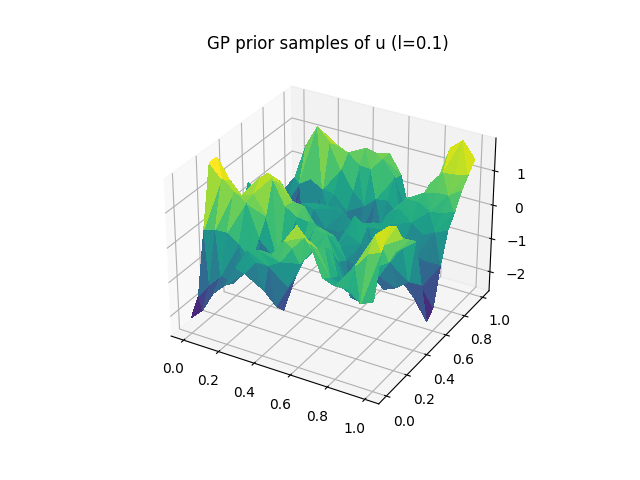
\includegraphics[width=\linewidth]{u-small.png}
		\caption{Small $l=0.1$}
	\end{subfigure}
	\begin{subfigure}{0.32\linewidth}
		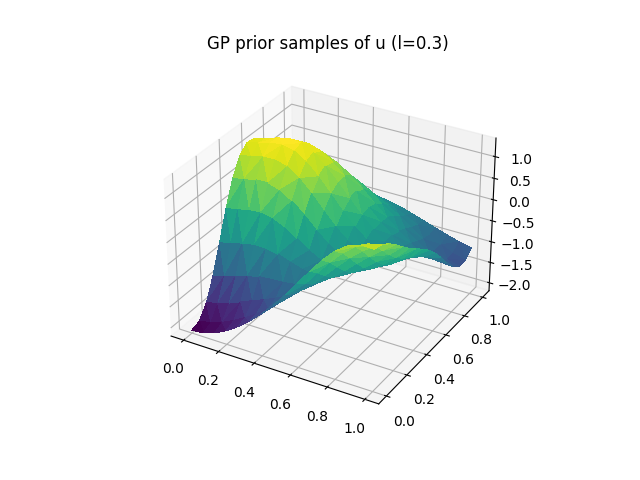
\includegraphics[width=\linewidth]{u-med.png}
		\caption{Medium $l=0.3$}
	\end{subfigure}
	\begin{subfigure}{0.32\linewidth}
		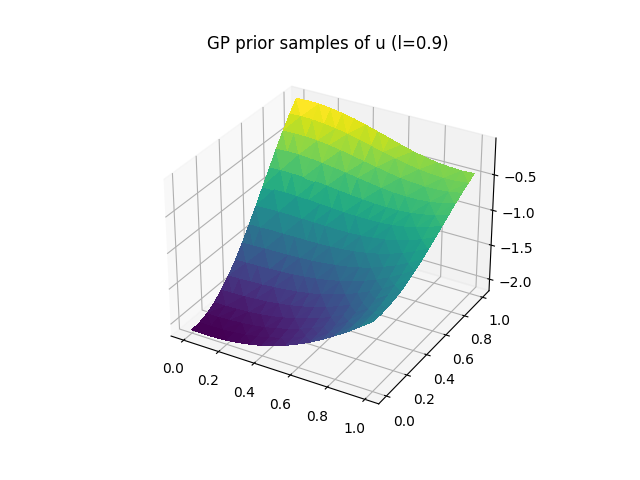
\includegraphics[width=\linewidth]{u-big.png}
		\caption{Large $l=0.9$}
	\end{subfigure}
	\caption{Samples from GP prior for varying length scales ($D=16$)}
	\label{fig:l-effect}
\end{figure}

We now proceed to make $M$ random draws (denoted by the $M \times 1$ vector $\vbold$) from these samples $\ubold$ with additive Gaussian noise $\epsbold \sim \Ncal(0, I)$. The subsampling factor $f$ is defined as $f \coloneqq N / M$. The draws can be computed as follows:
%
\begin{equation}
	\vbold = G \ubold + \epsbold
	\label{eqn:v-defn}
\end{equation}

Where $G$ is an $M \times N$ matrix with a single one in each row in a random location (without repetition) and rest zeros. The result is that the observations $\vbold$ are a jumbled subsample of $\ubold$ with additive noise $\epsbold$. We can plot the data overlaid on the original prior samples by simply matching each entry of $\vbold$ back to the coordinate it was selected from. The result is plotted on figure \ref{fig:v-on-u}.
%
\begin{figure}[!h]
	\centering
	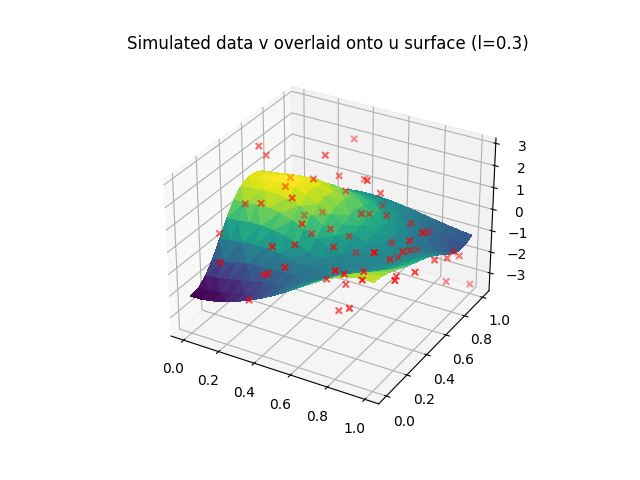
\includegraphics[width=\figwidth]{v-overlay.png}
	\caption{$\vbold$ (red crosses) overlaid on $\ubold$-surface ($f=4, D=16, l=0.3$)}
	\label{fig:v-on-u}
\end{figure}

We observe $M=N/f=16^2/4=64$ samples contained in the $\vbold$ vector. These are equally likely to appear above or below the $\ubold$-surface as the noise has zero mean. The noise variance for each data-point is of similar magnitude to the variation in the surface ($\sigma^2 = 1$) so some crosses appear relatively far away from the surface. Moreover, as the subsampling is random, the $\vbold$-points appear at randomly chosen (but distinct) locations X-Y plane.

\subsection{Log probabilities and MCMC}

We assume that we have realised a set of observations $\vbold$ and it is now our job to determine probability distributions for $\ubold$ based on this information. As a matter of notation, we define the prior function $\pi(\cdot) \coloneqq p(\ubold=\cdot)$ and likelihood function $\lik(\cdot) \coloneqq \ln p (\vbold | \ubold = \cdot)$. Likewise, we define the posterior $\rho(\cdot) \coloneqq p(\ubold=\cdot | \vbold)$.

The log prior can be calculated simply, through manipulation of the Gaussian pdf:
%
\begin{align}
	\ln \pi (\wbold) &= \ln \Ncal(\wbold; 0, C) \nonumber \\
	&= \ln \frac{1}{(2\pi)^{N/2} |C|^{1/2}} \exp \left( - \frac{1}{2} \wbold^T C^{-1} \wbold \right) \nonumber \\
	&= - \left( \frac{N}{2} \ln 2\pi + \frac{1}{2} \ln |C| + \frac{1}{2} \wbold^T C^{-1} \wbold \right)
	\label{eqn:log-prior}
\end{align}

Likewise, $\vbold | \ubold$ is also a Gaussian such that $\vbold |\ubold \sim \Ncal(G\ubold, I)$ (see equation \ref{eqn:v-defn}). By comparison with the form of equation \ref{eqn:log-prior}, we can jump straight to the log-likelihood, noting that $\ln |I| = 0$:
%
\begin{equation}
	\ln \lik(\wbold) = - \left( \frac{M}{2} \ln 2 \pi + \frac{1}{2} \left(\vbold - G\wbold \right)^T \left(\vbold - G\wbold\right)\right)
	\label{eqn:log-likelihood}
\end{equation}

From these it is trivial to determine the log-posterior from Bayes' rule:
%
\begin{align}
	\rho(\wbold) &\propto \pi(\wbold) \cdot \lik(\wbold) \nonumber \\
	\therefore \ln \rho(\wbold) &= \ln \pi(\wbold) + \ln \lik(\wbold) + \textrm{const}
\end{align}

It is important to note that, $\wbold$ is simply a dummy variable. We can simplify this notation further by defining $\Rho \coloneqq \ln \rho + \textrm{const}$, $\Pi \coloneqq \ln \pi$ and $\loglik \coloneqq \ln \lik$. The constant can be chosen to give us:
%
\begin{equation}
	\Rho(\omegabold) = \Pi(\omegabold) + \loglik(\omegabold)
	\label{eqn:log-posterior}
\end{equation}

\subsubsection{Gaussian Random Walk - Metropolis Hastings (GRW-MH)}

Armed with the log-posterior (equation \ref{eqn:log-posterior}), observations $\vbold$ and observation matrix $G$, we can now apply the Gaussian Random Walk Metropolis-Hastings algorithm to draw samples of $\ubold$ from the posterior. We start with an initial estimate drawn from the prior $\ubold^{(0)} \sim p(\ubold) = \Ncal(\ubold; 0, C)$. For simplicity we use the symbol $\zetabold$ to denote a fresh sample drawn from the prior $\pi \sim \Ncal(0, C)$. It is computed by applying a Cholesky decomposition to the covariance matrix $C$ and multiplying a standard Gaussian vector $\zbold \sim \Ncal(0, I)$. As such:
%
\begin{equation}
	\zetabold = C^{1/2} \zbold
	\label{eqn:zeta}
\end{equation}

To emphasise, every time $\zetabold$ appears in an equation we draw a fresh sample according to equation \ref{eqn:zeta}. We then pick a symmetric proposal distribution to sequentially generate samples. Given a sample $\ubold^{t}$ we generate a proposal $\wbold^{(t)}$ as follows:
%
\begin{equation}
	\wbold^{(t)} \coloneqq \ubold^{(t)} + \beta \zetabold
\end{equation}

Where $\beta$ is a hyperparameter that controls the step-size of each iteration. As our proposal distribution is symmetric, the acceptance probability $\alpha^{(t)} \coloneqq \alpha(\ubold^{(t)}, \wbold^{(t)})$ simplifies to the ratio of posteriors (with an upper bound of 1):
%
\begin{equation}
	\alpha(\ubold, \wbold) \coloneqq \min \left( \frac{\rho(\wbold)}{\rho(\ubold)}, 1 \right)
\end{equation}

It may be more natural to deal in log of this value:
%
\begin{equation}
	\ln \alpha^{(t)} = \min \left(\Rho(\wbold^{(t)}) - \Rho(\ubold^{(t)}), 0\right)
\end{equation}

Note that the constant term in the $\Rho$ definition cancels. Naturally, we can sample a uniform random variable $U \sim \mathcal{U}(0, 1)$ and compare to $\alpha^{(t)}$:
%
\begin{align}
	p(U < \alpha) &= \alpha \nonumber \\
	\therefore p(\ln U < \ln \alpha) &= \alpha
\end{align}

The algorithm for GRW-MH is given in algorithm \ref{alg:grw-mh}.
%
\begin{algorithm}
	\caption{Gaussian Random Walk - Metropolis Hastings}
	\label{alg:grw-mh}
\begin{algorithmic}
	\State $\ubold^{(0)} \gets \zetabold$
	\For{$t \in \{0, 1 \cdots T-1\}$}
	\State $\wbold^{(t)} \gets \ubold^{(t)} + \beta \zetabold$ \Comment{Generate proposal}
	\State $\ln \alpha^{(t)} \gets \min \left(\Rho(\wbold^{(t)}) - \Rho(\ubold^{(t)}), 0\right)$
	\State $U^{(t)} \gets \sim \mathcal{U}(0,1)$ \\
	\If {$\ln U^{(t)} \leq \ln \alpha^{(t)}$}
		\State $\ubold^{(t+1)} \gets \wbold^{(t)}$ \Comment{Proposal accepted}
	\Else
		\State $\ubold^{(t+1)} \gets \ubold^{(t)}$ \Comment{Proposal rejected}
	\EndIf
	\EndFor
\end{algorithmic}
\end{algorithm}

As our algorithm depends only on the difference of the posteriors, there is no need to compute the constant term. This massively speeds up computation.

\subsubsection{Preconditioned Crank-Nicholson (pCN)}

Preconditioned Crank-Nicholson is rather similar, except we choose a subtly different proposal distribution:
%
\begin{equation}
	\omegabold^{(t)} \coloneqq \sqrt{1 - \beta^2} \ubold^{(t)} + \beta \zetabold
\end{equation}

This changes the form of our acceptance probability subtly by exchanging the log-posterior $\Rho$ for the log-likelihood $\loglik$. The rest of the algorithm is broadly unchanged (see algorithm \ref{alg:pCN}).
%
\begin{algorithm}
	\caption{preconditioned Crank-Nicholson}
	\label{alg:pCN}
	\begin{algorithmic}
		\State $\ubold^{(0)} \gets \zetabold$
		\For{$t \in \{0, 1 \cdots T-1\}$}
		\State $\wbold^{(t)} \gets \sqrt{1 - \beta^2} \ubold^{(t)} + \beta \zetabold$ \Comment{Generate proposal}
		\State $\ln \alpha^{(t)} \gets \min \left(\loglik(\wbold^{(t)}) - \loglik(\ubold^{(t)}), 0\right)$
		\State $U^{(t)} \gets \sim \mathcal{U}(0,1)$ \\
		\If {$\ln U^{(t)} \leq \ln \alpha^{(t)}$}
		\State $\ubold^{(t+1)} \gets \wbold^{(t)}$ \Comment{Proposal accepted}
		\Else
		\State $\ubold^{(t+1)} \gets \ubold^{(t)}$ \Comment{Proposal rejected}
		\EndIf
		\EndFor
	\end{algorithmic}
\end{algorithm}

A huge advantage of pCN compared to GRW-MH is that we do not need to compute the prior probability for each proposal. This massively speeds up computation.

\subsubsection{Method comparison}

We run both algorithms for $T=10^4$ iterations and $\beta=0.2$. The algorithm returns the set $\{ \ubold^{(t)} \}_{t=1}^{T}$ which can be averaged to return a Monte-Carlo estimate of $\ubold$ denoted $\hat{\ubold}$:
%
\begin{equation}
	\hat{\ubold} = \frac{H}{T-B} \sum_{k=1}^{(T - B)/H} \ubold^{(B + ki)}
\end{equation}

The parameters $B$ and $H$ refer to the burn-in time and thinning rate respectively. This ensures that the estimate is unbiased and adjacent samples are uncorrelated. Choosing these parameters optimally is a report in itself. $B$ is chosen to be at least greater than the time it takes the Markov chain to reach a stationary distribution (can be estimated by plotting the sample magnitude with respect to iteration). $H$ is chosen by looking at the autocorellation of the generated samples and choosing an offset for which it is close to zero. We choose these to be $B=100$ and $H=5$ (justifications omitted for the sake of brevity).

We plot the estimated surface $\hat{\ubold}$ predicted by each algorithm in figure \ref{fig:u-estimate}. However, this plot is not very easy to interpret as both look broadly similar. Instead, we prefer to plot the absolute error surface $|\hat{\ubold} - \ubold|$ as that better visualises the accuracy of the predictions.
%
\begin{figure}[!h]
	\centering
	\begin{subfigure}{0.32\linewidth}
		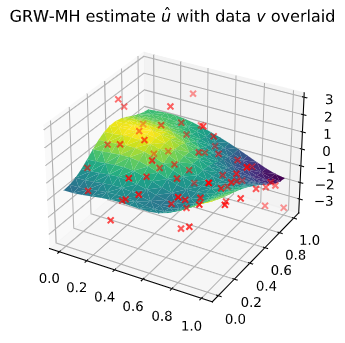
\includegraphics[width=\linewidth]{grw-mh-estimate.png}
		\caption{GRW-MH estimate}
		\label{fig:grw-estimate}
	\end{subfigure}
	\begin{subfigure}{0.31\linewidth}
		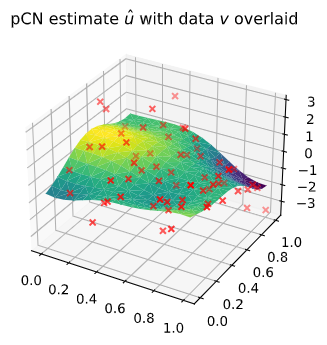
\includegraphics[width=\linewidth]{pcn-estimate.png}
		\caption{pCN estimate}
		\label{fig:pcn-estimate}
	\end{subfigure}
	\caption{Monte Carlo estimate errors ($D=16, T=10^4, \beta=0.2$)}
	\label{fig:u-estimate}
\end{figure}

The absolute error is plotted on figures \ref{fig:grw-err} and \ref{fig:pcn-err}. The error surface for each algorithm has a broadly similar shape (the mean absolute error is marginally higher for pCN). Indeed, by comparison with figure \ref{fig:v-2d}, the regions of high error are those in areas of sparse available data $\vbold$. This is to be expected as we cannot make a confident prediction in areas where we have few data-points.
%
\begin{figure}[!h]
	\centering
	\begin{subfigure}{0.32\linewidth}
		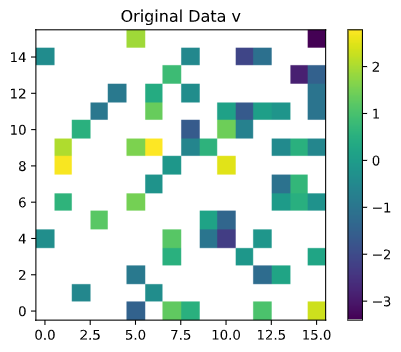
\includegraphics[width=\linewidth]{v-2d.png}
		\caption{Data $v$ projected onto X-Y plane}
		\label{fig:v-2d}
	\end{subfigure}
	\begin{subfigure}{0.32\linewidth}
		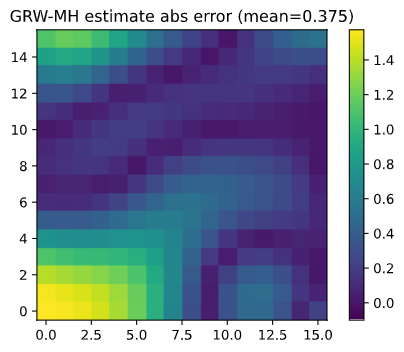
\includegraphics[width=\linewidth]{grw-mh-err.png}
		\caption{GRW-MH absolute error $|\hat{\ubold} - \ubold|$}
		\label{fig:grw-err}
	\end{subfigure}
	\begin{subfigure}{0.32\linewidth}
		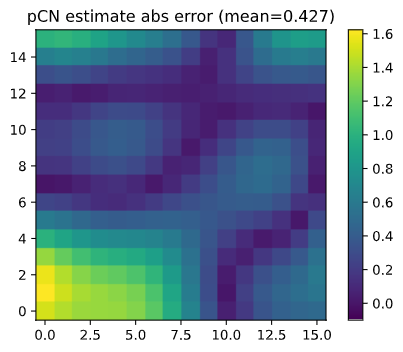
\includegraphics[width=\linewidth]{pcn-err.png}
		\caption{pCN absolute error $|\hat{\ubold} - \ubold|$}
		\label{fig:pcn-err}
	\end{subfigure}
	\caption{Monte Carlo estimate errors ($D=16, T=10^4, \beta=0.2$)}
	\label{fig:abs-error}
\end{figure}

The acceptance rate is an important measure of the wastefulness of the algorithm. We tabulate it in table \ref{tab:acceptance} for a range of grid-sizes $D$ and step-sizes $\beta$.
%
\begin{table}[!h]
	\centering
	\begin{tabular}{cc | cccc}
		Acceptance Rate    &    & \multicolumn{3}{c}{$\beta$}                    &  \\
		(GRW-MH $|$ pCN)       &    & 0.04          & 0.2           & 1.0            &           \\ \hline
		\multirow{2}{*}{D} & 4  & 0.932 $|$ 0.973 & 0.692 $|$ 0.886 & 0.054 $|$ 0.302 &           \\
		& 16 &   0.694 $|$ 0.851      &  0.097  $|$ 0.498         &    0.000 $|$  0.010  & 
	\end{tabular}
\caption{Acceptance rate for GRW-MH $|$ pCN algorithms for varying $\beta, D$}
\label{tab:acceptance}
\end{table}

Comparing the two algorithms, pCN has a higher acceptance for all tested scenarios. Higher dimensional spaces (larger $D$) necessarily have lower acceptance rates as there are more degrees of freedom so it is less likely that a random walk will move in a direction that increases the posterior (or likelihood for pCN). The acceptance rate for both algorithms decreases as $\beta$ increases. Nevertheless, having $\beta$ too low runs the risk of falling into a local optimum as there is insufficient energy to escape shallow wells. Therefore, it is less likely to converge to the true global optimum.

\subsection{Probit classification}

The model is now extended to work on a probit classification problem. The data $\vbold$ is put through a sign function to give the vector $\tbold$, such that $t_i \coloneqq \textrm{sign}(v_i)$. As such the likelihood has the following form:
%
\begin{align}
	p(t_i = 1 | \ubold) &= p(v_i > 0 | \ubold) \nonumber \\
	&= p([G\ubold]_i + \epsilon_i > 0) \nonumber \\
	&= p(-\epsilon_i < [G\ubold]_i ) \nonumber \\
	&= \Phi([G\ubold]_i)
\end{align}

Where $\Phi(\cdot)$ is the standard Gaussian CDF (as $-\epsilon_i \sim \epsilon_i \sim \Ncal(0,1)$). Conversely, for the case $t_i = -1$ the likelihood is given by:
%
\begin{align}
	p(t_i = -1 | \ubold) &= 1 - p(t_i = 1 | \ubold) \nonumber \\
	&= 1 - \Phi([G\ubold]_i) \nonumber \\
	&= \Phi(-1 \cdot [G\ubold]_i)
\end{align}

This means we can simplify the expression for $t_i \in {-1, 1}$, leading to:
%
\begin{equation}
	p(t_i | \ubold_i) = \Phi(t_i \cdot [G\ubold]_i)
\end{equation}

We can extend this easily to find the likelihood $\lik(\cdot)$\footnote{Note that for simplicity we are not changing notation and all previous symbols in the $\vbold$ problem will retain their meaning for the $\tbold$ problem} of the latent variables $\ubold$ given the whole vector of observations $\tbold$:
%
\begin{align}
	\lik(\ubold) &= p(\tbold | \ubold) \nonumber \\
	&= \prod_{i=1}^{M} p(t_i | \ubold) \nonumber \\
	&= \prod_{i=1}^{M} \Phi(t_i \cdot [G\ubold]_i)
\end{align}

The second line arises from the fact that $t_i \indep t_j | \ubold$ or more specifically given $G\ubold$. This a direct result of equation \ref{eqn:v-defn} as the noise terms $\epsilon_i$ are mutually independent. However, instead we find it easier to deal with the log-likelihood $\loglik(\cdot) \coloneqq \ln \lik(\cdot)$ as this turns the multiplication into a summation:
%
\begin{align}
	\loglik(\ubold) &= \sum_{i=1}^{M} \ln \Phi(t_i \cdot [G\ubold]_i) \nonumber \\
	&= \mathbf{1}^T \left[ \ln \Phi(\tbold \odot G\ubold) \right]
	\label{eqn:log-lik-probit}
\end{align}

Where $\odot$ denotes element-wise multiplication of vectors, $\ln$ and $\Phi$ are extended to operate element-wise also and $\mathbf{1}$ is simply the vector of all-ones. This form in equation \ref{eqn:log-lik-probit} is very easy to implement using numpy as it is vectorised. With this log-likelihood function we can sample from the posterior $p(\ubold | \tbold)$ using pCN. From these samples we can perform a Monte Carlo estimate of the true class assignments for any $t^*_j$ not restricted to the subsampling imposed by $G$. The Monte-Carlo estimate is computed as follows:
%
\begin{align}
	p(t^*_j = 1 | \tbold) &= \int p(t^* = 1, \ubold | \tbold) d\ubold \nonumber \\
	&= \int p(t^* = 1 | \ubold) p(\ubold | \tbold) d\ubold \nonumber \\
	&\approx \frac{1}{T} \sum_{t=1}^{T} p \left( t^* = 1 | \ubold^{(t)} \right) \nonumber \\
	&= \frac{1}{T} \sum_{t=1}^{T} \Phi \left( u^{(t)}_j \right)
\end{align}

Where each $\ubold^{(t)}$ denotes a sample drawn from the posterior $p(\ubold | \tbold)$ as is the case under pCN. As we are bypassing the subsampling matrix $G$ both the $\tbold^*$ and $\ubold^*$ vectors are indexed by the same variable $j$, labelling position on the finite 2-D grid on the X-Y plane. We can quickly compute the vector of probabilities by dropping the $j$ dependence to give equation \ref{eqn:t-mc-estimate}:
%
\begin{equation}
	p(\tbold^* | \tbold) \approx \frac{1}{T} \sum_{t=1}^{T} \Phi \left( \ubold^{(t)} \right)
	\label{eqn:t-mc-estimate}
\end{equation}
\subsection{Length scale inference}

\section{Spatial Data}

\subsection{Poisson Likelihood}

\subsection{Monte Carlo Estimation}

\textbf{Words}: XX

\end{document}
